% -*- LaTeX -*- Time-stamp: <02/12/06 15:21:12 ptr>

\documentclass[a4paper]{article}

\usepackage[T1]{fontenc}
\usepackage{pslatex}
\usepackage{pstricks}
\usepackage[dvips]{epsfig}
%\usepackage[dvipdf]{graphics}
\usepackage[dvips]{graphics}
\usepackage[american]{babel}

\title{Performance Estimation of Sockios Library}
\author{Petr Ovtchenkov}

\begin{document}

\maketitle

\section{Computers and Networks}

\begin{enumerate}
  \item AMD Athlon XP 1500+ (dual) under Linux (2.4.17),
        Ethernet card: Intel Corp. 82557 [Ethernet Pro 100].\label{fort}
  \item Intel Pentium 133MHz under Linux (2.4.17),
        Ethernet card: RealTek RTL8139 Fast Ethernet.\label{oldnavy}
  \item Intel Pentium III 803MHz under Solaris 8,
        Ethernet card: Intel 82558/82559 [EEPRO 100+].\label{ermine}
\end{enumerate}

Network between systems \ref{fort} and \ref{oldnavy}: 100Mb Ethernet,
UTP level 5, point-to-point (no hubs, routers,
switches or other devices between computers).

\section{Compilers}

On all systems was used GNU gcc 3{.}1{.}1 ($C{+}{+}$ or $C$, depends
upon programs).

\section{Tests Goals}

Compare performance of sockios library. Detect problems and ways for
possible solutions.

\section{Tests description}

\begin{figure}
  \begin{center}
    % \input test.pstex_t
    \epsfig{file=test.eps,width=5in}
  \end{center}
  \caption{Test time diagram. Shown only two experiment from ten.\ref{TimeDiagram}.}
\end{figure}

\begin{enumerate}
  \item Start server.
  \item Start client.
  \item Client connect to the server and send $n$ blocks of size $b$;
        server read all sended by client data and write ones into one
        buffer of size $b$, data overwritten.
\end{enumerate}

This procedure repeat $10$ times. During tests we collect some statistic
data: client and server user CPU time, system CPU time and elapsed (real) time.
Then we find mean values and dispersion. So we can estimate the real
load from client and server programs in the real environments.

In case of client and server run on different computers, we start server on
the local system, login via \texttt{ssh} on remote hoste and start here client.
Login via ssh is done under \texttt{ssh-agent}, to avoid manual password typing.

We compare results of sockios library with ``ideal'' times from
C-written programs with restricted functionality (no buffering, no multiple
clients processing on server side, no multithreading).

Due to ``time'' function has different options and output format on Linux
and Solaris, we use program \texttt{time} from this
bundle\footnote{Portabilty note: system should has \texttt{wait3} function.}.
By the way this function use high-precision time measure.

Client connect to the server and send $n$ blocks of size $b$ via TCP/IP protocol.
The numbers $n$ and $b$ choose so that $n b = 52428800$ (i.e. client send
to the server $50$M). We make estimations for $5$ cases:
\begin{itemize}
  \item many small messages ($b = 32$);
  \item basic message size ($b = 1024$, i.e. $1$K);
  \item messages of page size ($b = 4096$, i.e. $4$K);
  \item large messages ($b = 1048576$, i.e. $1$M);
  \item huge messages ($b = 52428800$, i.e. $50$M).
\end{itemize}

\section{Results}

\begin{figure}
  \begin{center}
    \input p1.tex
    % \epsfig{file=p1.eps}
  \end{center}
  \caption{Local Loopback, sockios: system \ref{fort}.}
\end{figure}

\begin{figure}
  \begin{center}
    \input p2.tex
  \end{center}
  \caption{Network, sockios:
           systems \ref{fort} (server) and \ref{oldnavy} (client).}
\end{figure}

\begin{figure}
  \begin{center}
    \input p3.tex
  \end{center}
  \caption{Local Loopback, sockios: system \ref{ermine}.}
\end{figure}

\begin{figure}
  \begin{center}
    \input p4.tex
  \end{center}
  \caption{Local Loopback, restricted code on $C$: system \ref{fort}.}
\end{figure}

\begin{figure}
  \begin{center}
    \input p5.tex
  \end{center}
  \caption{Local Loopback, restricted code on $C$: system \ref{ermine}.
           Test results for block size $32$ skiped here; one has 
           mean elapsed time $128.637$s, client system mean 
           time $6.088$s, client user mean time $1.133$s, server system
           mean time $114.252$s, server user mean time $1.951$s.\label{local-C-ermine}}
\end{figure}

Really, systems can send/receive only $64$K at once
(default settings, local loopback, \texttt{read}/\texttt{write} system calls
without return). This fact we see on the figure~\ref{local-C-ermine}:
with tiny packets and unbuffered data system has so bad performance,
I removed this point from picture, to avoid too small scale of other results.


\end{document}
